
\begin{figure*}[!htb]
  \centering
  \begin{subfigure}[t]{0.3\textwidth}
	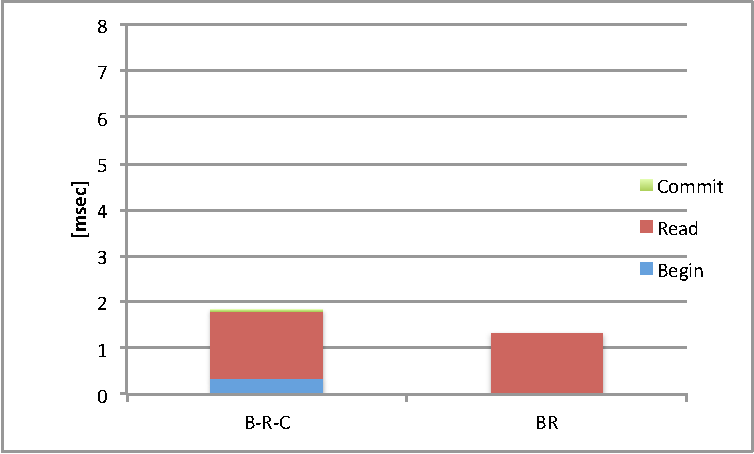
\includegraphics[width=\textwidth]{figs/read_latency.pdf}
	\caption[]{Read Latency}
  \end{subfigure}
  \begin{subfigure}[t]{0.3\textwidth}
	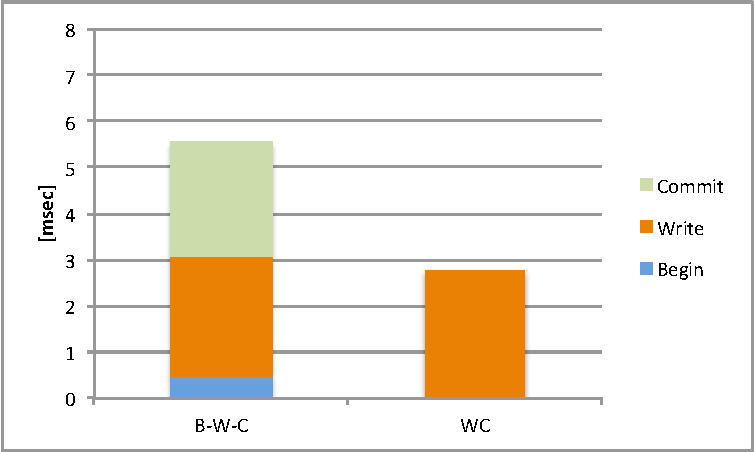
\includegraphics[width=\textwidth]{figs/write_latency.pdf}
	\caption[]{Write Latency}
  \end{subfigure}	
  \begin{subfigure}[t]{0.3\textwidth}
	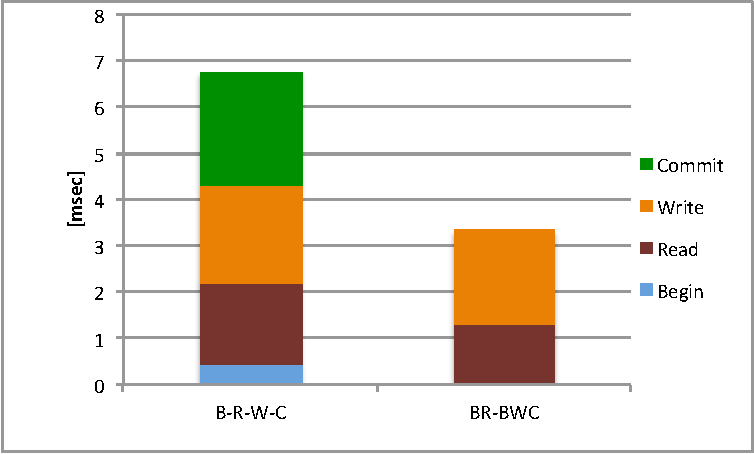
\includegraphics[width=\textwidth]{figs/rmw_latency.pdf}
	\caption[]{Read Modify Write Latency}
  \end{subfigure}			
  \caption{Latency}\label{fig:latency}
  \label{fig:latency}
\end{figure*}


\paragraph{Methodology}
In order to evaluate local transaction performance, we set up a 3 node Hbase cluster loaded with 20M keys that take up 50GB of storage.
-TSO
-load on TSO and hbase that create random transactions
-ycsb version that does full transactions

\paragraph{Results}
Results are shown in Figure~\ref{fig:latency}

